\documentclass{ctexart}
\usepackage[]{amsmath}
\usepackage[]{graphicx}
\usepackage[]{algorithm}
\usepackage[]{algorithmicx}
\usepackage[]{algpseudocode} 
\usepackage[]{natbib} 
\begin{document}
\title{最优化第四次上机作业}
\author{王恒亮 \quad 学号:1601210102}
\date{}
\maketitle
本次实现了解决Minimax Problems的三种方法,分别为Least pth Method\cite{Charalambous1979}, Smoothing Method\cite{Xu2001}和Adaptive Smoothing Method\cite{Polak2003}。以下分别介绍算法及程序实现,实验结果及分析。
\section{算法及程序实现}
\subsection{Least pth Method}
Least pth Method 主要通过优化U函数来解决Minimax问题,U函数的定义如下:
\begin{equation}
	\label{eq:ufun}
	U(x,u,p,\xi)=\left\{
		\begin{aligned}
			M(x,\xi)&(\sum_{i\in S(x,\xi)}{u_i(\frac{f_i(x)-\xi}{M(x,\xi)})^q})^{1/q}, &\text{for} M(x,\xi) \neq 0,\\
				       &0, &\text{for} M(x,\xi) = 0
		\end{aligned}\right.
\end{equation}

其中:
\begin{align}
	u_i \geq 0\quad \text{and} \quad\sum_{i\in I}{u_i} = 1\\
	M(x, \xi) = \max_{i\in I}{(f_i(x) - \xi)}
\end{align}

算法的框架如下:
\begin{description}
	\item[步1] 取$p>1, \xi^{(1)} =0,u_i^{(1)}=1,i\in I,x=x^0,r=1$
	\item[步2] 固定$u,p,\xi$,在公式\ref{eq:ufun}中对x取极小,最优解设为$x^r$
	\item[步3] 更新$u$
	\[u^{r+1}_i\frac{v_i^{r+1}}{\sum_{j\in I}{v_j^{r+1}}}, i\in I\]
	其中:
	\[v_{i}^{r+1}=\left\{
		\begin{aligned}
			u_i^r(\frac{f_i(x^r)-\xi}{M(x^r,\xi)})^{q-1}, \text{for}\quad i \in S(x^r,\xi)\\
			0, \text{for}\quad i\in I - S(x^r, \xi)
		\end{aligned}\right.\]
	\[S(x^r, \xi)=\left\{
		\begin{aligned}
			&\{i|f_i(x)-\xi>0,i\in I\}, &\text{if} M(x^r,\xi) \geq 0\\
			&I, &\text{if} M(x^r,\xi) <0
		\end{aligned}\right.\]
	\item[步4] 更新$\xi$
	\[\xi^{r+1} = \left\{
		\begin{aligned}
			&\xi^r + M(x^r, \xi^r) , &\text{if} M(x^r, \xi) < 0\\
			&\xi^r + \lambda M(x^r, \xi^r), &\text{otherwise.}
		\end{aligned}\right.\]
	\item[步5] 更新$p, p = cp, c\geq 1$,转至步2
\end{description}

在实现中,除了计算出了最优点和最优点的函数值之外,还记录了迭代次数,函数调用次数,具体的参数设置将在结果中说明。
\subsection{Smoothing Method}
Smoothing Method是将Minimax问题转化为优化近似函数$f(x,\mu)$,其定义如下:
\[f(x,\mu) = \mu\ln\sum_{i=1}^{m}{\exp(\frac{f_i(x)}{\mu})}\]
对于$f(x,\mu)$的优化使用牛顿法求出下降方向,使用Armijo准则找到步长,在每步迭代后会更新$\mu, \mu = \beta\mu$。对于$f(x,\mu)$的函数,梯度和Hessian矩阵的计算如下:
$$
\begin{aligned}
	f(x^k,\mu_k)=&f(x^k)+\mu_k\ln\sum_{i=1}^{m}{exp(\frac{f_i(x^k)-f(x^k)}{\mu_k})}\\
	\bigtriangledown_xf(x,\mu)=&\sum_{i=1}^m{\lambda_i(x,\mu)\bigtriangledown f_i(x)}\\
\bigtriangledown^2_xf(x,\mu)=&\sum_{i=1}^m(\lambda_i(x,\mu)\bigtriangledown^2f_i(x)+\frac{1}{\mu}\lambda_i(x,\mu)\bigtriangledown f_i(x)\bigtriangledown f_i(x)^T)\\
			& -\frac{1}{\mu}(\sum_{i=1}^{m}\lambda_i(x,\mu)\bigtriangledown f_i(x))(\sum_{i=1}^m{\lambda_i(x,\mu)\bigtriangledown f_i(x)})^T\\
	\lambda_i(x^k,\mu_k) =& \frac{exp(\frac{f_i(x^k)-f(x^k)}{\mu_k})}{\sum_{j=1}^{m}{exp(\frac{f_j(x^k)-f(x^k)}{\mu_k})}}
\end{aligned}
$$
\subsection{Adaptive Smoothing Method}
Adaptive Smoothing Method是在Smoothing Method的基础对算法做了改进,主要解决了在$\mu\rightarrow 0$时产生的ill-condition问题。Adaptive Smoothing Method将Minimax问题转化为优化公式\ref{eq:adasmooth}。
\begin{equation}
\label{eq:adasmooth}
\Phi_p(x)=\log(\sum_{j\in Q}{(\exp(pf^j(x)))/p}
\end{equation}
具体算法如下:
\begin{description}
	\item[步1] 取$i=0,k=0,\gamma = 1$
	\item[步2] 设$\Phi_{p_i,xx}(x_i)$是Hessian矩阵R的Cholesky修正,$c(R)$为R的条件数的倒数,则若$\Phi_{p_i,xx}(x_i)$正定且$c(R)\geq k_1,p_i\leq k_3$,转步3,若$\Phi_{p_i,xx}(x_i)$正定且$c(R)\geq k_1$且$\Phi_{p_i,xx}(x_i)$的最大特征值$\sigma_{p_i,max}(x_i)$满足$\sigma_{p_i,max}\leq k_2$,转步3,否则转步4
	\item[步3] $h_{p_i}(x_i) = -\Phi_{p_i,xx}(x_i)^{-1}\bigtriangledown\Phi_{p_i}(x_i)$,转步5
	\item[步4] $h_{p_i}(x_i) = -\bigtriangledown_{p_i}\Phi(x_i)$
	\item[步5] 计算步长\\
	\[\lambda_{p_i}(x_i) = \max_{l\in N}\{\beta^l|\Phi_{p_i}(x_i+\beta^lh_{p_i}(x_i))-\Phi_{p_i}(x_i)\leq \alpha\beta^l\langle\bigtriangledown\Phi_{p_i}(x_i),h_{p_i}(x_i)\rangle\}\]
\item[步6] $x_{i+1} = x_i + \lambda_{p_i}(x_i)h_{p_i}(x_i)$
\item[步7] 若$|\bigtriangledown\Phi_{p_i}(x_i)|^2\leq \tau(p_i)$,转步8,否则设$p_{i+1}=2p_i, i=i+1$,转步2
\item[步8] 若$p^*\leq \hat{p},\gamma=1$,其中$p^*$满足$\epsilon_a(p_i)\leq |\bigtriangledown\Phi_{p^*}(x_i)|^2\leq \epsilon_b(p_i)$,则设$\gamma=\max\{2,(\hat{p}+2)/(k+1)\}, p_{i+1}=\gamma(k+2),k=k+1, i=i+1$,否则设$p_{i+1}=\gamma(k+2),k=k+1,i=i+1$,转步2
\end{description}
\section{实验结果及分析}
本次实验分别在Xu\cite{Xu2001}中实验中第2,3题中的函数和\cite{Charalambous1979}中的Digital filter example滤波器函数进行结果测试。实验结果如下:
\subsection{Xu\cite{Xu2001}中例子2}
问题描述如下:
\[minimize_{i=1,2,3}f_i(x)\]
其中:
$$
\begin{aligned}
	f_1(x) &= x_1^4+x_2^2\\
	f_2(x) &= (2-x_1)^2 + (2-x_2)^2\\
	f_3(x) &= 2\exp(-x_1+x_2)
\end{aligned}$$
初始点取值为$(1,-0.1)$,最优点取值为$(1,1)$。各个方法的数值结果如表\ref{tab:xu2}。
\begin{table}[htpb]
	\centering
	\caption{Xu中例子2}
	\label{tab:xu2}
	\begin{tabular}{c c c c}
	\hline
	方法 & $|f^*-f|$ & 迭代次数 & 函数调用次数 \\\hline
	Least pth & $7.2482\times 10^{-5}$ & 24 & 72 \\
	Smooth Method & $4.3247\times 10^{-7}$ &28 & 57\\
	Adaptive Smooth & $4.7311\times 10^{-5}$ & 43 & 167 \\
	\hline
	\end{tabular}
\end{table}
\subsection{Rosen-Suzuki Problem}
问题描述为:
$$\begin{aligned}
	F(x)&=x_1^2+x_2^2+2x_3^2+x_4^2-5x_1-5x_2-21x_3+7x_4\\
	g_2(x)&=-x_1^2-x_2^2-x_3^2-x_4^2-x_1+x_2-x_3+x_4+8\\
	g_3(x)&=-x_1^2-2x_2^2-x_3^2-2x_4^2+x_1+x_4+10\\
	g_4(x)&=-x_1^2-x_2^2-x_3^2-2x_1+x_2+x_4+5\\
	f_2&=F(x)-\alpha_2g_2(x)\\
	f_3&=F(x)-\alpha_3g_3(x)\\
	f_4&=F(x)-\alpha_4g_4(x)\\
	\alpha_2&=\alpha_3=\alpha_4=10
\end{aligned}$$
初始值取值为$(0,0,0,0)$,最优解$x^*=(0,1,2,-1)$。各个方法的数值结果如表\ref{tab:rspro}。
\begin{table}[htpb]
	\centering
	\caption{Rosen-Suzuki Problem数值结果}
	\label{tab:rspro}
	\begin{tabular}{c c c c}
	\hline
	方法 & $|f^*-f|$ & 迭代次数 & 函数调用次数 \\\hline
	Least pth & $3.6745\times 10^{-5}$ & 13 & 39\\
	Smooth Method & $1.4665\times 10^{-10}$ & 47 & 147\\
	Adaptive Smooth & $7.5858\times 10^{-11}$ &41 &113 \\
	\hline
	\end{tabular}
\end{table}
\subsection{Digital filter example}
滤波器函数主要参考了\cite{Charalambous1974Minimax}中的函数。滤波器函数定义如下:
$$\begin{aligned}
|H(x,\theta)|=&A\prod_{k=1}^{K}{\frac{N_k}{D_k}}\\
		&A\prod_{k=1}^{K}{(\frac{1+a_k^2+b_k^2+2b_k(2\cos^2\theta-1)+2a_k(1+b_k)\cos\theta}{1+c_k^2+d_k^2+2d_k(2\cos^2\theta-1)+2c_k(1+d_k)\cos\theta})^{1/2}}
\end{aligned}$$
其中:
$$\begin{aligned}
	x&=[a_1,b_1,\cdots,c_K,d_k,A]^T\\
	n&=4K+1
\end{aligned}$$
则对其求导可得$|H(x,\theta)|$对$x$中各个变量的导数。
$$\begin{aligned}
	\frac{\partial{|H(x,\theta)|}}{\partial{a_j}}&=\frac{|H(x,\theta)|}{N_j^2}[a_j+(1+b_j)\cos\theta]\\
	\frac{\partial{|H(x,\theta)|}}{\partial{b_j}}&=\frac{|H(x,\theta)|}{N_j^2}[-1+2\cos^2\theta+a_j\cos\theta+b_j]\\
	\frac{\partial{|H(x,\theta)|}}{\partial{c_j}}&=-\frac{|H(x,\theta)|}{D_j^2}[c_j+(1+d_j)\cos\theta]\\
	\frac{\partial{|H(x,\theta)|}}{\partial{d_j}}&=\frac{|H(x,\theta)|}{D_j^2}[-1+2\cos^2\theta+c_j\cos\theta+d_j]\\
	\frac{\partial{|H(x,\theta)|}}{\partial{A}}&=\frac{|H(x,\theta)|}{A}
\end{aligned}$$
再对导数求导可以得到其Hessian矩阵如下:
$$\begin{aligned}
	\frac{\partial^2{|H(x,\theta)|}}{\partial{a_j^2}}&=\frac{|H(x,\theta)|}{N_j^4}(1-b_j)^2\sin^2\theta\\
	\frac{\partial^2{|H(x,\theta)|}}{\partial{a_j}\partial{a_k}}&=\frac{|H(x,\theta)|}{N_j^2N_k^2}[a_j+(1+b_j)\cos\theta][a_k+(1+b_k)\cos\theta],(k\neq j)\\
	\frac{\partial^2{|H(x,\theta)|}}{\partial{a_j}\partial{b_j}}&=\frac{|H(x,\theta)|}{N_j^4}(a_j(\cos\theta+1)+\sin^2\theta(2\cos\theta-2b_j\cos\theta-a_jb_j))\\
	\frac{\partial^2{|H(x,\theta)|}}{\partial{a_j}\partial{b_k}}&=\frac{|H(x,\theta)|}{N_j^2N_k^2}[a_j+(1+b_j)\cos\theta][-1+2\cos^2\theta+a_k\cos\theta+b_k],(k\neq j)\\
	\frac{\partial^2{|H(x,\theta)|}}{\partial{a_j}\partial{c_k}}&=-\frac{|H(x,\theta)|}{N_j^2D_k^2}[a_j+(1+b_j)\cos\theta][c_k+(1+d_k)\cos\theta]\\
	\frac{\partial^2{|H(x,\theta)|}}{\partial{a_j}\partial{d_k}}&=-\frac{|H(x,\theta)|}{N_j^2D_k^2}[a_j+(1+b_j)\cos\theta][-1+2\cos^2\theta+c_j\cos\theta+d_j]\\
	\frac{\partial^2{|H(x,\theta)|}}{\partial{a_j}\partial{A}}&=\frac{|H(x,\theta)|}{N_j^2A}[a_j+(1+b_j)\cos\theta]\\
	\frac{\partial^2{|H(x,\theta)|}}{\partial{b_j^2}}&=\frac{|H(x,\theta)|}{N_j^4}(a_j+2\cos\theta)^2\sin^2\theta\\
	\frac{\partial^2{|H(x,\theta)|}}{\partial{b_j}\partial{b_k}}&=\frac{|H(x,\theta)|}{N_j^2N_k^2}(-1+2\cos^2\theta+a_j\cos\theta+b_j)(-1+2\cos^2\theta+a_k\cos\theta+b_k),(k\neq j)\\
	\frac{\partial^2{|H(x,\theta)|}}{\partial{b_j}\partial{c_k}}&=-\frac{|H(x,\theta)|}{N_j^2D_k^2}[-1+2\cos^2\theta+a_j\cos\theta+b_j][c_k+(1+d_k)\cos\theta]\\
	\frac{\partial^2{|H(x,\theta)|}}{\partial{b_j}\partial{d_k}}&=-\frac{|H(x,\theta)|}{N_j^2D_k^2}[-1+2\cos^2\theta+a_j\cos\theta+b_j][-1+2\cos^2\theta+c_j\cos\theta+d_j]\\
	\frac{\partial^2{|H(x,\theta)|}}{\partial{b_j}\partial{A}}&=\frac{|H(x,\theta)|}{N_j^2A}[-1+2\cos^2\theta+a_j\cos\theta+b_j]\\	
	\frac{\partial^2{|H(x,\theta)|}}{\partial{c_j^2}}&=\frac{|H(x,\theta)|}{D_j^4}(2(c_j+(1+d_j)\cos\theta)^2-(1-d_j)^2\sin^2\theta)\\
	\frac{\partial^2{|H(x,\theta)|}}{\partial{c_j}\partial{d_j}}&=\frac{|H(x,\theta)|}{D_j^4}(4\cos\theta-5c_j^2\cos\theta+3c_j-10c_j\cos^2\theta-2d_j\cos\theta\\
	&-2d_j^2\cos\theta-2d_j\cos^3\theta-6\cos^3\theta+2c_jd_j\cos\theta-3c_jd_j-6c_jd_j\cos^2\theta)\\
	\frac{\partial^2{|H(x,\theta)|}}{\partial{c_j}\partial{d_k}}&=\frac{|H(x,\theta)|}{D_j^2D_k^2}[c_j+(1+d_j)\cos\theta][-1+2\cos^2\theta+c_k\cos\theta+d_k],(k\neq j)\\
\end{aligned}$$
$$
\begin{aligned}
	\frac{\partial^2{|H(x,\theta)|}}{\partial{c_j}\partial{A}}&=\frac{|H(x,\theta)|}{D_j^2A}[a_j+(1+b_j)\cos\theta]\\
	\frac{\partial^2{|H(x,\theta)|}}{\partial{d_j^2}}&=\frac{|H(x,\theta)|}{D_j^4}[3(-1+2\cos^2\theta+c_j\cos\theta+d_j)^2-D_j^2]\\
	\frac{\partial^2{|H(x,\theta)|}}{\partial{d_j}\partial{A}}&=\frac{|H(x,\theta)|}{D_j^2A}[-1+2\cos^2\theta+c_j\cos\theta+d_j]\\	
	\frac{\partial^2{|H(x,\theta)|}}{\partial A^2}&=0
\end{aligned}$$
在实验中逼近函数为$S(\phi) = |1-2\phi|,0\leq\phi\leq 1$,误差函数为$e(x,\phi)=|H(x,\theta)-S(\phi)|$,问题转化为$\min_x\max_{0\leq\Phi\leq 1}{|e(x,\Phi)|}$。$\Phi$的取值如下:
$$\begin{aligned}
	\Phi &= 0.0, 0.05(0.01);\quad i=1,\cdots,6,\\
	\Phi &= 0.07, 0.46(0.03);\quad i=7,\cdots,20,\\
	\Phi &= 0.5, 0.54(0.04);\quad i=21,22\\
	\Phi &= 0.57,0.67(0.1);\quad i=23,24\\
	\Phi &= 0.63,0.93(0.03);\quad i=25,\cdots,35,\\
	\Phi &= 0.95,1.0(0.01);\quad i=36,\cdots,41
\end{aligned}$$
初始点设为$(0,1,0,-0.15,0,-0.68,0,-0.72,0.37)$,最优解为$(0.,0.980039,0.$ $,-0.165771,0.,-0.767228,0.367900)$各个方法的数值结果如表\ref{tab:filter}。
\begin{table}[htpb]
	\centering
	\caption{滤波器数值结果}
	\label{tab:filter}
	\begin{tabular}{c c c c}
	\hline
	方法 & $|f^*-f|$ & 迭代次数 & 函数调用次数 \\\hline
	Least pth & 0.0064 & 7 &21 \\
	Smooth Method & 0.0086 & 26 & 105\\
	Adaptive Smooth &0.0078 &42 & 165 \\
	\hline
	\end{tabular}
\end{table}

三种方法的误差曲线图如图\ref{fig:leastpth},\ref{fig:xusmooth},\ref{fig:adasmooth}。
\begin{figure}[htpb]
	\centering
	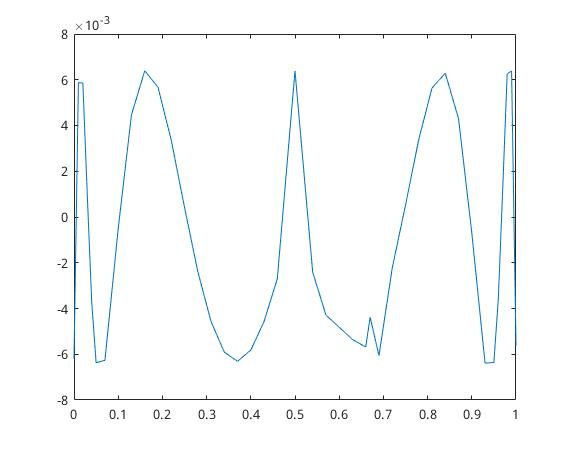
\includegraphics[width=0.8\linewidth]{pic/leastpth.jpg}
	\caption{Leastpth误差曲线}
	\label{fig:leastpth}
\end{figure}
\begin{figure}[htpb]
	\centering
	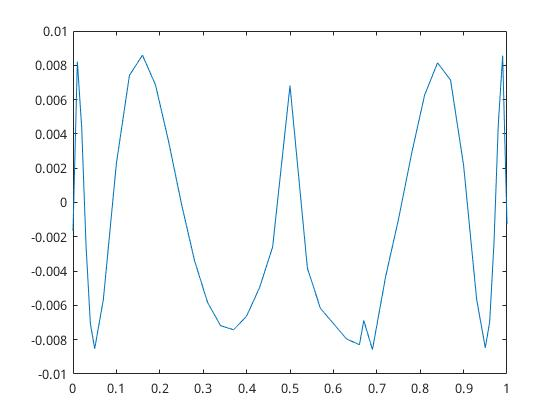
\includegraphics[width=0.8\linewidth]{pic/xusmooth.jpg}
	\caption{Smooth Method误差曲线}
	\label{fig:xusmooth}
\end{figure}
\begin{figure}[htpb]
	\centering
	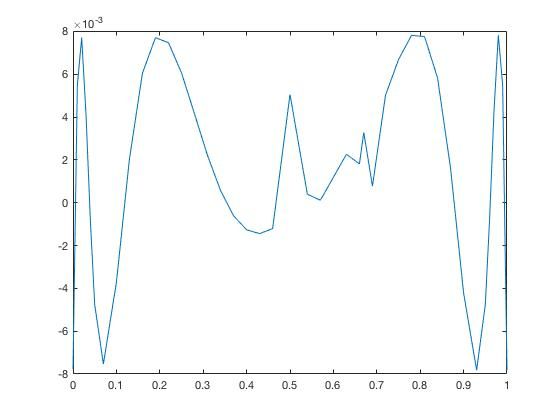
\includegraphics[width=0.8\linewidth]{pic/adasmooth.jpg}
	\caption{Adaptive Smooth误差曲线}
	\label{fig:adasmooth}
\end{figure}
\subsection{结果分析}
在实验中,可以看出以下几点:
\begin{itemize}
\item Least pth方法在几种情况是比较稳定的,而且在几组实验中的迭代次数和函数调用次数均是最少的,而且在滤波器的例子中达到了最优的效果。
\item Smooth Method方法实现比较简单,同时在三组实验中也达到了较不错的效果。
\item Adaptive Smooth Method方法虽然是在Smooth Method的基础上进行改进的,但是并不能一定比Smooth Method的效果好,但在多数情况下能够比Smooth Method在更少的迭代次数和函数调用次数下达到更好的效果。方法的稳定性不如Least pth方法。
\end{itemize}
\bibliographystyle{plain}
\bibliography{refer}
\end{document}
